\documentclass[a4paper,11pt]{article}
\usepackage{amsmath,amsthm,amsfonts,amssymb,amscd,amstext,vmargin,graphics,graphicx,tabularx,multicol} 
\usepackage[francais]{babel}
\usepackage[utf8]{inputenc}  
\usepackage[T1]{fontenc} 
\usepackage{pstricks-add,tikz,tkz-tab,variations}
\usepackage[autolanguage,np]{numprint} 

\setmarginsrb{1.5cm}{0.5cm}{1cm}{0.5cm}{0cm}{0cm}{0cm}{0cm} %Gauche, haut, droite, haut
\newcounter{numexo}
\newcommand{\exo}[1]{\stepcounter{numexo}\noindent{\bf Exercice~\thenumexo} : \marginpar{\hfill /#1}}
\reversemarginpar


\newcounter{enumtabi}
\newcounter{enumtaba}
\newcommand{\q}{\stepcounter{enumtabi} \theenumtabi.  }
\newcommand{\qa}{\stepcounter{enumtaba} (\alph{enumtaba}) }
\newcommand{\initq}{\setcounter{enumtabi}{0}}
\newcommand{\initqa}{\setcounter{enumtaba}{0}}

\newcommand{\be}{\begin{enumerate}}
\newcommand{\ee}{\end{enumerate}}
\newcommand{\bi}{\begin{itemize}}
\newcommand{\ei}{\end{itemize}}
\newcommand{\bp}{\begin{pspicture*}}
\newcommand{\ep}{\end{pspicture*}}
\newcommand{\bt}{\begin{tabular}}
\newcommand{\et}{\end{tabular}}
\renewcommand{\tabularxcolumn}[1]{>{\centering}m{#1}} %(colonne m{} centrée, au lieu de p par défault) 
\newcommand{\tnl}{\tabularnewline}

\newcommand{\bmul}[1]{\begin{multicols}{#1}}
\newcommand{\emul}{\end{multicols}}

\newcommand{\trait}{\noindent \rule{\linewidth}{0.2mm}}
\newcommand{\hs}[1]{\hspace{#1}}
\newcommand{\vs}[1]{\vspace{#1}}

\newcommand{\N}{\mathbb{N}}
\newcommand{\Z}{\mathbb{Z}}
\newcommand{\R}{\mathbb{R}}
\newcommand{\C}{\mathbb{C}}
\newcommand{\Dcal}{\mathcal{D}}
\newcommand{\Ccal}{\mathcal{C}}
\newcommand{\mc}{\mathcal}

\newcommand{\vect}[1]{\overrightarrow{#1}}
\newcommand{\ds}{\displaystyle}
\newcommand{\eq}{\quad \Leftrightarrow \quad}
\newcommand{\vecti}{\vec{\imath}}
\newcommand{\vectj}{\vec{\jmath}}
\newcommand{\Oij}{(O;\vec{\imath}, \vec{\jmath})}
\newcommand{\OIJ}{(O;I,J)}


\newcommand{\reponse}[1][1]{%
\multido{}{#1}{\makebox[\linewidth]{\rule[0pt]{0pt}{20pt}\dotfill}
}}

\newcommand{\titre}[5] 
% #1: titre #2: haut gauche #3: bas gauche #4: haut droite #5: bas droite
{
\noindent #2 \hfill #4 \\
#3 \hfill #5

\vspace{-1.6cm}

\begin{center}\rule{6cm}{0.5mm}\end{center}
\vspace{0.2cm}
\begin{center}{\large{\textbf{#1}}}\end{center}
\begin{center}\rule{6cm}{0.5mm}\end{center}
}



\begin{document}
\pagestyle{empty}
\titre{Contrôle n 3 }{Nom :}{Prénom :}{2015/2016}{Classe}


\exo{2} Cours \\


\bmul{2}

Sur la figure ci-contre, les points A, R, G, I, L, E sont alignés, de même que les points P, O, I, D, S.\\
A partir du codage, citer tous les segments ayant pour milieu le point I :\\

\noindent \reponse[1]

\columnbreak

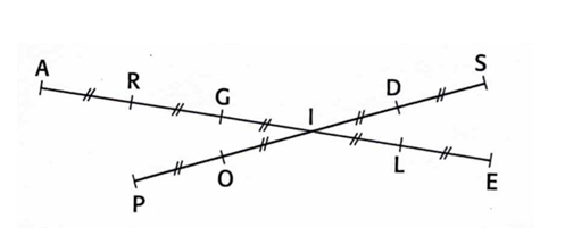
\includegraphics[scale=1]{milieu.eps} 

\emul

\exo{4} Encadrer les abscisses des points entre deux nombres décimaux en utilisant les traits de graduation les plus proches.\\


\begin{center}

\includegraphics[scale=1]{droite.eps} 
\end{center}

\bmul{2}

..... < abscisse de A < ....

\columnbreak

..... < abscisse de B < ....


\emul

\medskip

\begin{center}
\includegraphics[scale=1]{dtes.eps} 
\end{center}

\bmul{2}

..... < abscisse de C < ....

\columnbreak

..... < abscisse de D < ....


\emul



\exo{3,5}\\


\includegraphics[scale=1]{point.eps} 
\vspace*{1.5cm}

\initq 
\q Tracer un segment [AB] de longueur 7,8 cm.\\

\q Placer sur ce segment le point M à 2,3 cm du point A.\\

\q Calculer la longueur MB :	MB = ................................................................................... \\

\q Placer le milieu I du segment [AB].\\

\q Calculer les longueurs AI et IM :\\	

AI = ....................................................................	IM = ....................................................................\\

\q Placer le point N à l'aide du compas pour que B soit le milieu du segment [MN].\\

\newpage

\exo{4}

\bmul{2}

\initq \q Tracer (d), la médiatrice du segment [KL].\\
    Que peut-on dire des droites (d) et (KL) ?\\
\reponse[2]\\

\q Placer sur (d) un point A tel que : A $\notin$ [KL].\\

\q Tracer la droite (d’) perpendiculaire à 
la droite (d) passant par A.\\

\columnbreak


\includegraphics[scale=1]{segment.eps} 

\emul



\q Que peut-on dire des droites (d’) et (KL) ?\\
\reponse[1]\\

Citer la propriété utilisée :\\
\reponse[2]\\

\exo{2,5}   Pour chaque question, entourer la bonne réponse :

\begin{flushleft}
\includegraphics[scale=1]{tablrau.eps} 
\end{flushleft}

\exo{1,5}Entourer les nombres qui sont plus proches de 1,4 que de 1,5.\\

\begin{center}
\begin{tabular}{|c|c|c|c|c|c|}
\hline 
\hspace*{0.1cm}  1,476 & 1,432 \hspace*{0.1cm} & \hspace*{0.1cm} $\dfrac{1468}{1000}$ \hspace*{0.1cm}&\hspace*{0.1cm} $\dfrac{144}{100}$ \hspace*{0.1cm}&\hspace*{0.1cm} 1,4099 \hspace*{0.1cm} & \hspace*{0.1cm} $1 + \dfrac{457}{1000}$ \hspace*{0.1cm}\\ 
\hline 
\end{tabular} 
\end{center}

\exo{2,5}

Dans un collège les élèves sont, soit demi-pensionnaires (D.P.), soit externes. Parmi tous les élèves de 4ème, 110 sont externes. Chaque élève étudie au choix une deuxième langue : anglais, allemand ou espagnol. 

\initq \q Recopier et compléter le tableau :\\

\begin{center}
\begin{tabular}{|c|c|c|c|c|}
\hline 
 & Anglais & Allemand & Espagnol & Total \\ 
\hline 
D.P. &  &  & 60 & 130 \\ 
\hline 
Externes &  & 32 &  &  \\ 
\hline 
Total & 66 & 72 &  &  \\ 
\hline 
\end{tabular} 
\end{center}


\q Combien d'élèves étudient l'anglais en deuxième langue vivante ?\\
\reponse[1]\\

\q Combien d'externes ont anglais en deuxième langue vivante ?\\
\reponse[1]\\

\q A quoi correspond le nombre entouré dans le tableau ?\\
\reponse[1]\\

\exo{1,5} Bonus\\

Compléter les phrases suivantes :\\

\initq 
\q Les nombres décimaux ayant deux chiffres après la virgule compris entre 359,687 et 359,723 sont:\\ \reponse[1]

\q La valeur approchée par excès à l'unité est 243. La partie décimale est 0,17. Quel est ce nombre ?\\
\reponse[1]




\end{document}
